\chapter{Human Aware Robot Guide} % Main chapter title

\label{chapter:spencer} % Change X to a consecutive number; for referencing this chapter elsewhere, use \ref{ChapterX}

\lhead{Chapter 4. \emph{Human Aware Robot Guide}} % Change X to a consecutive number; this is for the header on each page - perhaps a shortened title



\section{Human-Aware Robot Guide}
\label{sec:case_study-spencer}
\subsection{Introduction}
\label{subsec:case_study-spencer-intro}
\subsubsection{Overview on the topic}
One interesting problem in human-robot interaction is developing robots able to guide humans, by offering a tour of attractions in an area or simply by helping to reach a destination.
A generic mobile robot platform should possess a vast set of skills, which includes advanced perception, motion planning, and task planning. These skills are not enough for a robot guide, which is deployed in highly dynamic human environments, and need to be complemented with human-aware behaviors.

%Examples
Different robot guides have been studied and developed, starting with pioneers like Rhino and Minerva \cite{thrun2000probabilistic}.  Few systems have actually been deployed for long period of time in human environments. Rackhman \cite{clodic2006rackham}, a museum guide with human-aware behaviors, is an example of such system, and has been deployed in a science museum for several months. Another example of robot guide was developed in \cite{bueno2011autonomous}, where the robot is integrated  in a smart museum environment, using virtual avatars with human-aware interfaces, associated to exhibitions, in order to convey information to users. After these first experiments, several researchers have tried to focus on the social aspects of the problem, which are especially important if the robot needs to offer information. Studies like \cite{yousuf2012development,evers2014development} focus on how the robot should address humans, concentrating on spatial relationships and on how the robot can convey information.

Building and using mental models of users is important in these scenarios, particularly if we are developing a proactive robot, which approaches people in order to offer its services, while monitoring their level of interest in the interaction. \cite{Jensen2005} presents an assessment of human-robot interaction during an exhibition, where perceptual and task related data are used to compute an internal state according to the scenario. With these information, the robot can compute a new emotional state and interact accordingly with users.
In \cite{rashed2015toward}, a robot guide is able to infer people's intention by studying their trajectories. The authors conducted experiments in a museum, managing to classify user trajectories in three categories and developing a method to identify participants that may need guidance. 

Recently, there has been emphasis on robot navigation algorithms that reason about human beings in the environment differently from other static or dynamic obstacles. Starting from proxemics, researchers have investigated explicit social signals, based on human-posture and the affordances of the environment, to improve the legibility of the robot's motions. For a detailed discussion on human-aware navigation algorithms we refer the readers to \cite{kruse2013human,rios-ijsr-2014}. Human-aware navigation in a museum situation was studied in \cite{samejima2015building}, where the authors build environmental maps, which include information learnt from human trajectories and postures, in order to plan safe paths that do not disturb humans present in the area. 

The robot guide scenario can become more complex if we consider not only single humans, but groups. Humans, in fact, tend to naturally form groups, which can be classified in different types, based on their size, on their level of cohesion, on their duration, and other factors \cite{forsyth2009group}.  Studying group formations is a complex problem, since the robot must be able to detect humans, which can be occluded in populated environments; and to model their social interactions, which can be ambiguous. One of the most powerful and expressive social cues is distance, used in different works to track social relationship, like \cite{luber2013multi}. 

\subsubsection{Motivations}
We believe that most robot guide systems are focusing on the social aspects of the problem, and on human-aware navigation, without fully considering the fundamental aspects of joint actions. Guiding is a collaborative task, where the robot does not need only to reach a destination, but also to ensure that its followers reach it, while providing a socially acceptable experience to them. In order to achieve this goal, the robot needs to constantly monitor its users, to adapt to their behaviors and to be ready to proactively help them.

The european project SPENCER \footnote{http://www.spencer.eu/} was born with the idea to study social awareness issues in human-robot interaction, and particularly in the application of a robot guide. This project aimed at joining complex robotic algorithms  with social signal processing, by modeling people not as objects, but as entities with relationships, social rules, and culturally diverse backgrounds. The final goal of the project was deploying a robot guide, in collaboration with the KLM airline\footnote{https://www.klm.com}, in the Schiphol airport of Amsterdam, performing user studies on real passengers to evaluate the validity of the system.

We applied our system to this framework, creating a human-aware robot guide which is able to lead a group of people to a destination. More particularly, the originality of our approach is that the robot is able to show both adaptive and a proactive behaviors. The robot will try, while guiding, to select a speed that pleases its users, when adapting, or to propose a new speed, using environmental and task related stimulus. Finally, our system will proactively try to engage members of the group if it detects they need assistance. 

\subsection{Building a Robot Guide}
\label{subsec:case_study-spencer-robot_guide}
In order to adapt our system to the robot guide scenario we had to enhance several modules, as shown in figure \ref{fig:case_study-spencer-architecture}: 
\begin{itemize}
\item The user is able to interact with the robot by using a tactile interface on its front. We updated our human interface to reflect the commands that the user is able to use.
\item In this scenario we are not really interested in the intention recognition skills that we developed in Chapter \ref{chapter:situation_assessment}. In an airport there are no complex sequence of actions that humans need to perform and we will evaluate users' intentions by their trajectories and the surrounding environment. We developed an Environment-Based Intention Situation Assessment module to enhance our Situation Assessment layer, presented in subsection \ref{subsec:case_study-spencer-intention}.  
\item Similarly, task planning and plan management is quite simple in this scenario. The robot will mostly vary its paths in the environment, using similar plans. We developed an A*-based task planner, which is able to find a path in a semantic map, to guide users to their destination, presented in subsection \ref{subsec:case_study-spencer-planning} 
\item The main work, in this application, has been creating a Collaborative Planner to guide users in a human-aware way. Using this planner, our robot is able to adapt itself to users' actions, or to proactively propose new behaviors. This planner is presented in subsection~\ref{subsec:case_study-spencer-collaborative_guide_planner}.
\end{itemize} 

\begin{figure}[ht!]
	\centering
	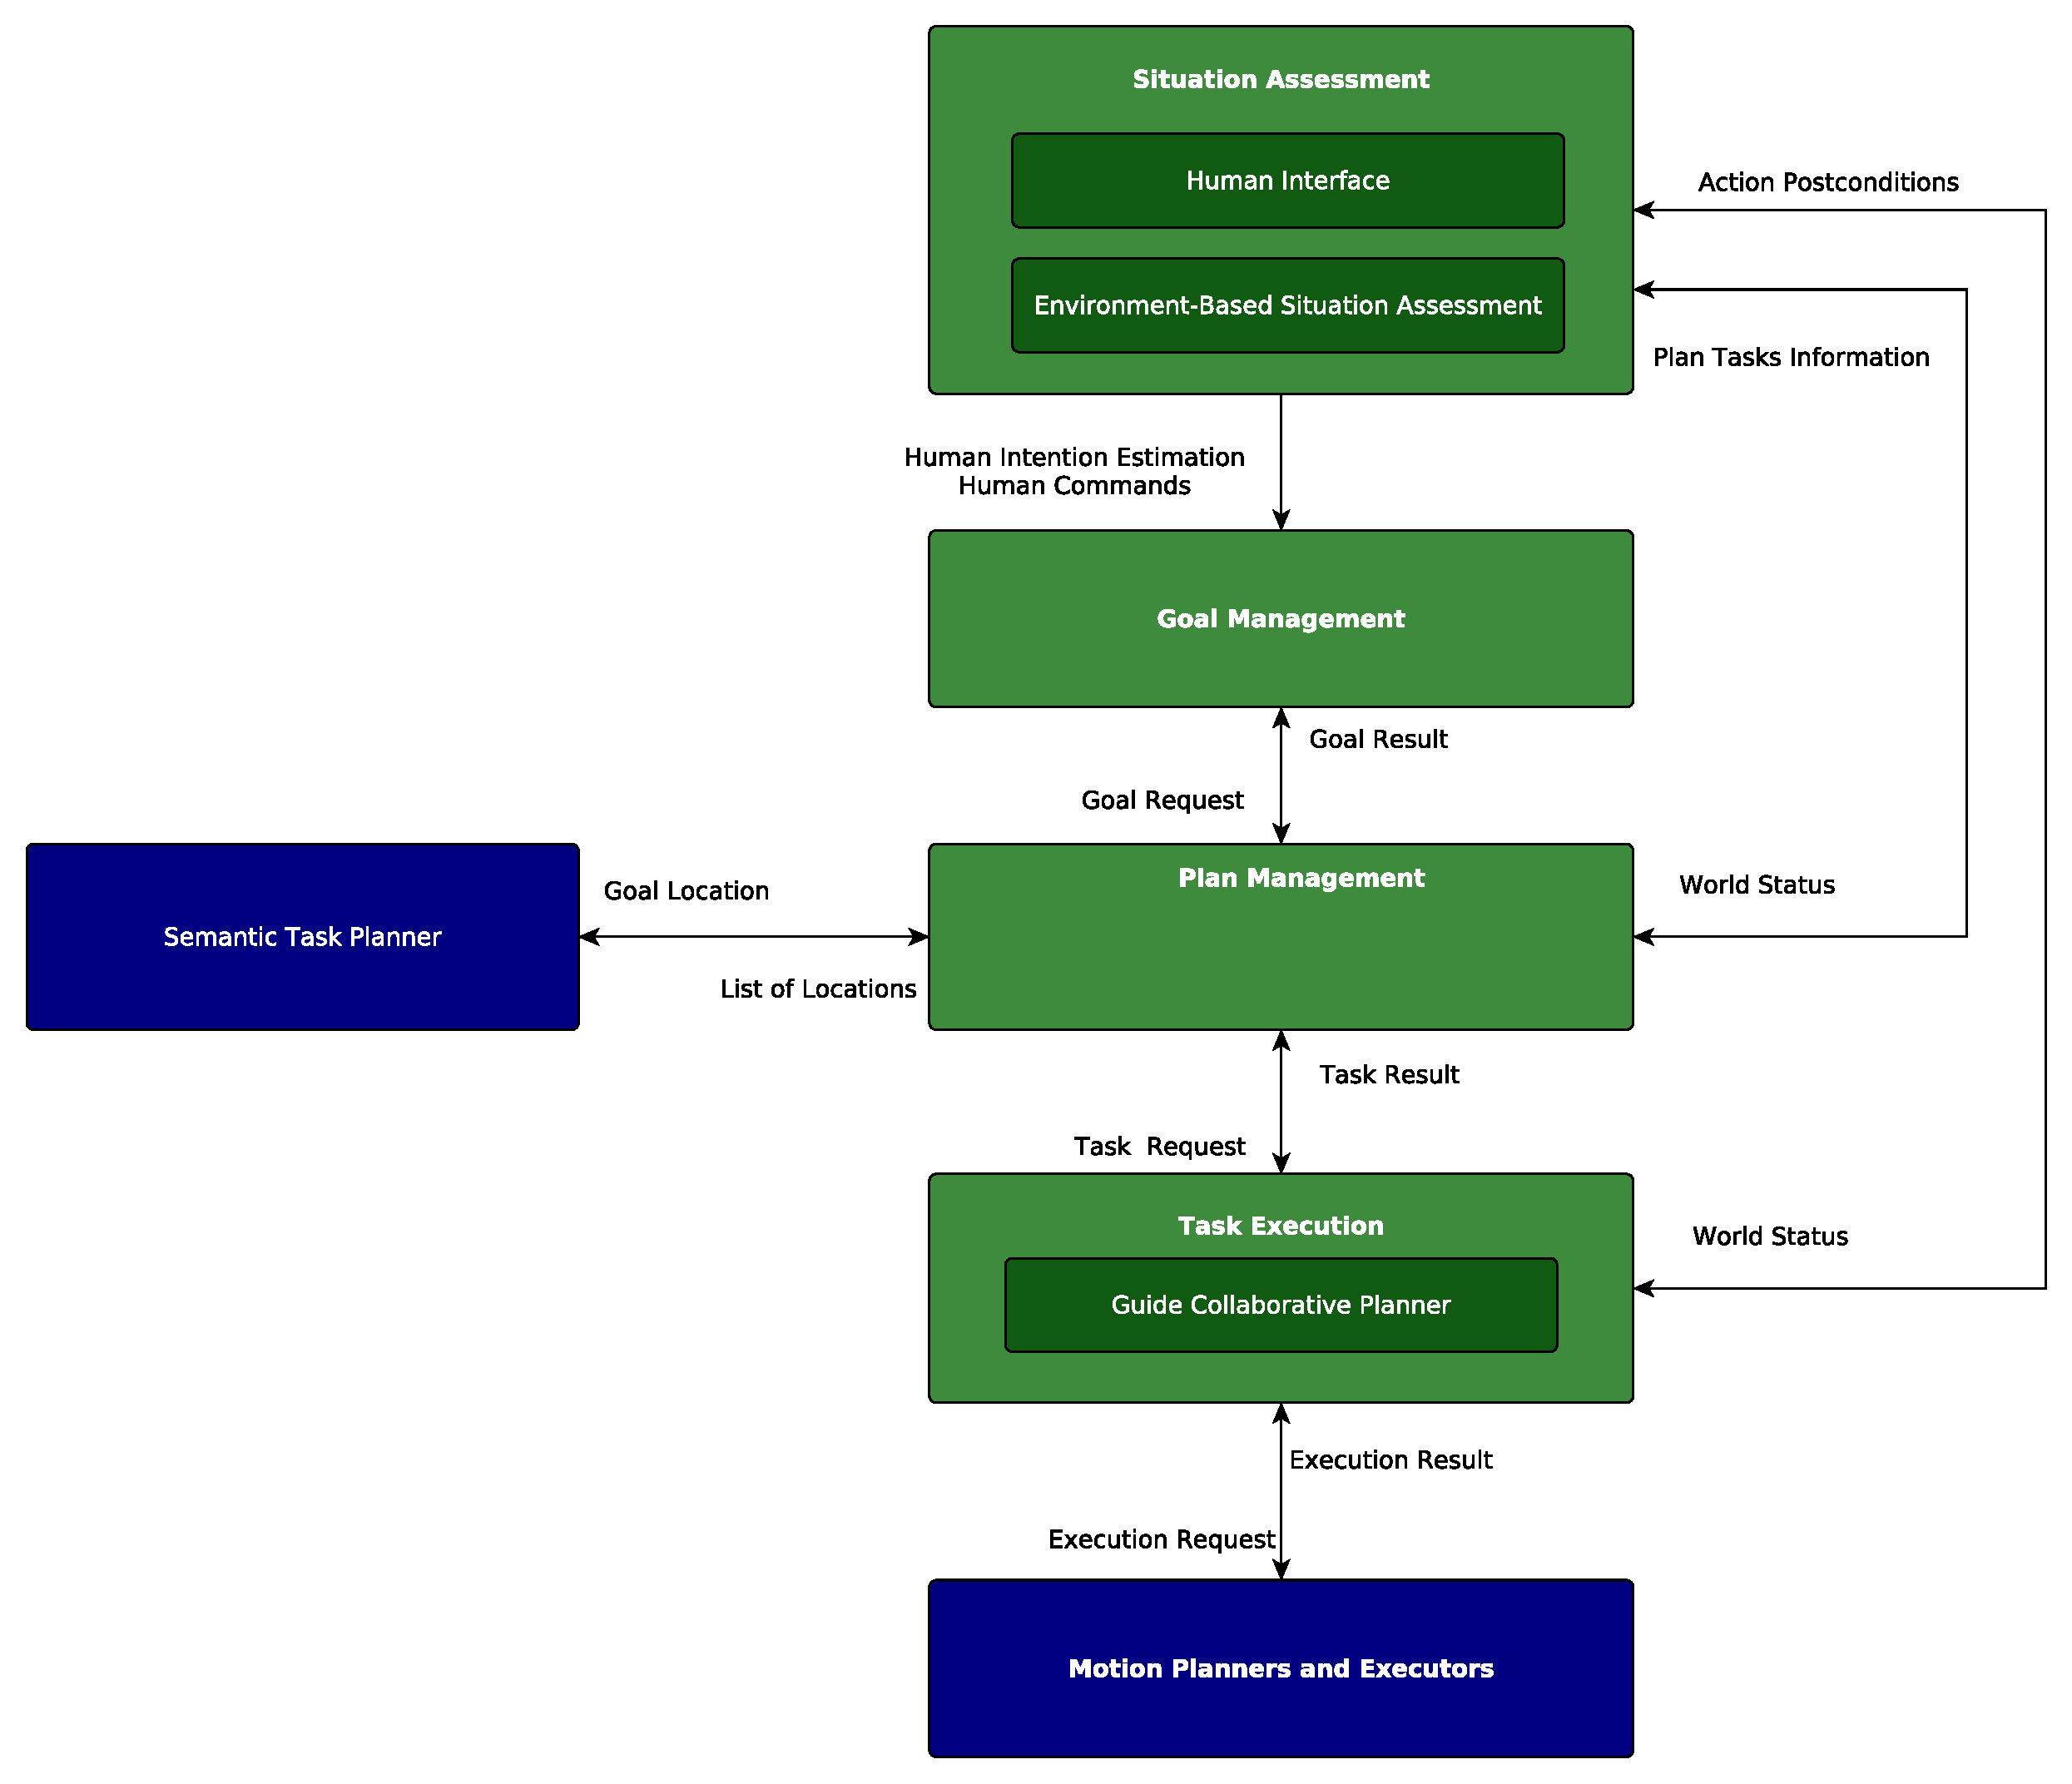
\includegraphics[scale=0.45]{img/case_study/spencer/architecture.pdf}
	\caption[Robot guide architecture]{This image shows the main layers of our architecture, represented as dark green rectangles, as shown in \ref{intro-system_overview}. In each layer, represented as light green rectangles, we show the modules that we modified or introduced in the robot guide scenario.}
	\label{fig:case_study-spencer-architecture}
\end{figure}

The system has been tested with different configurations, in laboratory experiments and in the Schipol airport, as shown in subsection \ref{subsec:case_study-spencer-lab_experiments} and \ref{subsec:case_study-spencer-airport}.

Parts of this section were presented in \cite{fiore2015adaptive}.

\subsection{Environment-Based Situation Assessment}
\label{subsec:case_study-spencer-intention}
There are many situations where, to properly reason on humans, we should link their movements and actions to the current environment. Imagine for example the case where we see a person oriented toward a screen. In an airport, we could infer from this observation that the person is looking at the screen, and perhaps in need of information. 

We introduced, in the Situation Assessment layer, the ability able to create activity areas in the environment and link them to different kind of computations. An activity area is a polygonal or circular area, which can be fixed or linked and updated with an entity's (object, human or robot) position. We studied and experimented two activity areas:

\begin{itemize}
\item Information Screen Area. This area, shown in figure \ref{fig:case_study-spencer-screen_area} is linked to information screens present in the environment. Using this information, the robot can recognize that humans are looking at the screen, and  start a proactive behavior, like approaching to offering help or information.
\item Touristic Point Area. These areas are linked to interesting sights and attractions in the environment. We can imagine, for example, to associate these areas to paintings, statues, or even rooms in a museum. Knowing that a human is in a touristic point area, and looking at an attraction, the robot could approach the human and tell him some interesting information about it.
\end{itemize}

\begin{figure}[ht!]
	\centering
	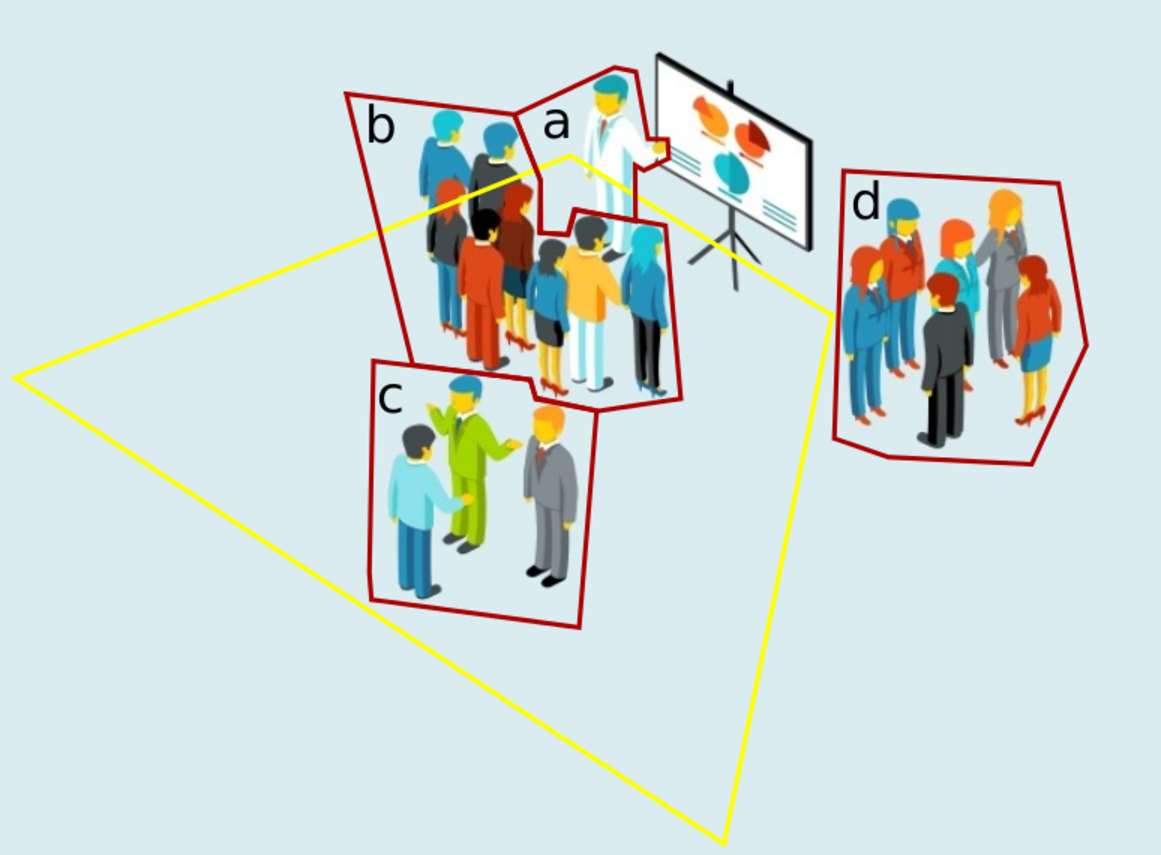
\includegraphics[scale=0.45]{img/case_study/spencer/environment_intention.pdf}
	\caption[Environment-Based Situation Assessment]{The Information Screen area used for environment-based intention recognition. The yellow polygon represents an area linked to the screen in the figure. Red polygons represent groups of person in the area. The person in group \textit{a} is in the screen area, but the robot will infer that he is not looking at the screen, since he is oriented in another direction. The persons in group \textit{b} are in the screen area and oriented toward the screen, so the robot infers that they are looking at it. The persons in group \textit{c} are not looking at the screen since they are either oriented in another direction or outside its area.}
	\label{fig:case_study-spencer-screen_area}
\end{figure}

\subsection{Task and Motion Planning Problems}
\label{subsec:case_study-spencer-planning}
To guide people in environments like museum or airports, the robot will need to navigate very large areas, which are often too big to efficiently perform motion planning. A solution to this problem is reducing the size of the area where the motion planner will compute its paths, splitting the navigation problem in a list of sub goals. The problem, with this approach,  is choosing the correct list of sub-goals to reach the final position.  To deal with this issue we implemented an A*-based task planner, which will choose a high-level path to be followed by the robot from a semantic map. This map is a hand-crafted graph, composed by different nodes, that represent parts of the environemt (corridors, elevator entrances, gates, etc.). Each node will be linked to a point in the real world. This task planner will, so, produce a list of coordinates usable by the motion planning layer. 

\begin{figure}[ht!]
	\centering
	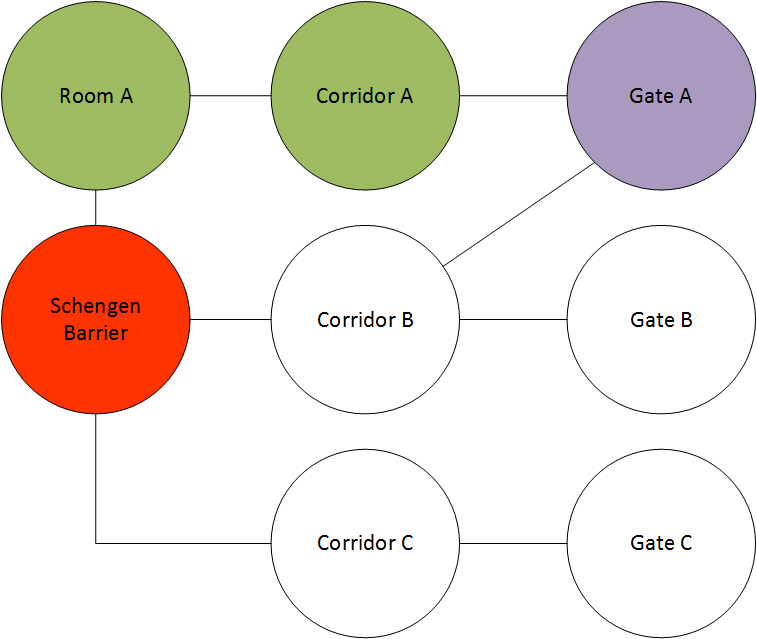
\includegraphics[scale=0.45]{img/case_study/spencer/ShengenTaskPlanner.png}
	\caption[Robot Guide Plan]{An example of plan computed in the robot guide scenario. The circles represent nodes in the semantic map. The purple node is the starting node of the plan. The red node is the goal. The green nodes represent intermediate nodes in the plan.}
	\label{fig:case_study-spencer-semantic_plan}
\end{figure}


A first way to manage this kind of plan is simply travelling to each calculated point, sending a goal to the motion planner for the next point every time the robot reaches its sub-destination. The problem with this approach is that the path followed by the robot might be very inefficient and not look natural.

Our solution was using a rolling window approach, shown in figure~\ref{fig:case_study-spencer-rolling_window}, where the motion planner will compute paths on a grid map centered on the robot, which will be updated with its position. In this way, the robot will send the next sub-goal in the calculated plan as soon as it is present in the rolling window, without waiting to reach the previous sub-goal. It is very important, with this approach to carefully select the nodes in the semantic maps so that the rolling window will contain at least two semantic nodes. If not, the motion planner would have to plan a path to a goal outside its grid map, which would generate an error.


\begin{figure}[ht!]
	\centering
	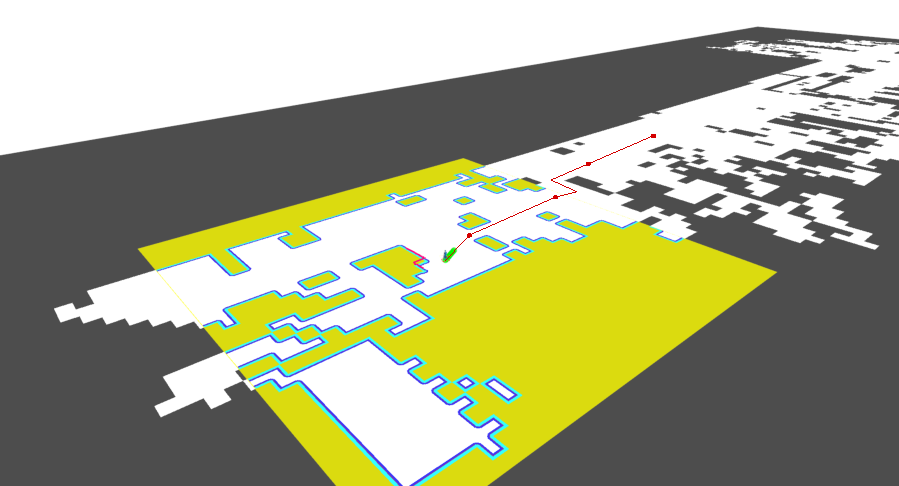
\includegraphics[]{img/case_study/spencer/rolling_window.pdf}
	\caption[Rolling window]{This figure shows the rolling window approach. The motion planner will compute robot paths in the grid represented by the yellow area, which is always centered on the robot. The red line and the red dots represent the sequence of goals calculated by the task planners. Each goal from this path is sent to the motion planner as soon as it is inside the window. The robot path does not pass through the closest node, since there is a further one in the rolling window.}
	\label{fig:case_study-spencer-rolling_window}
\end{figure}

\subsection{Collaborative Guide Planner }
\label{subsec:case_study-spencer-collaborative_guide_planner}

We developed a new collaborative planner to guide users to a destination. The planner is organized as a hierarchic MOMDP, as shown in figure \ref{fig:case_study-spencer-guide_planner} and is composed by several models:
\begin{itemize}
\item Guide Group Model. The main MOMDP of the hierarchy, responsible of choosing the main action performed by the robot.
\item Speed Adaptation Model. This model chooses if the robot should accelerate, decelerate, or keep the current speed.
\item Suspend Model. This module chooses which actions to execute when the users has stopped following.
\end{itemize}



\begin{figure}[ht!]
	\centering
	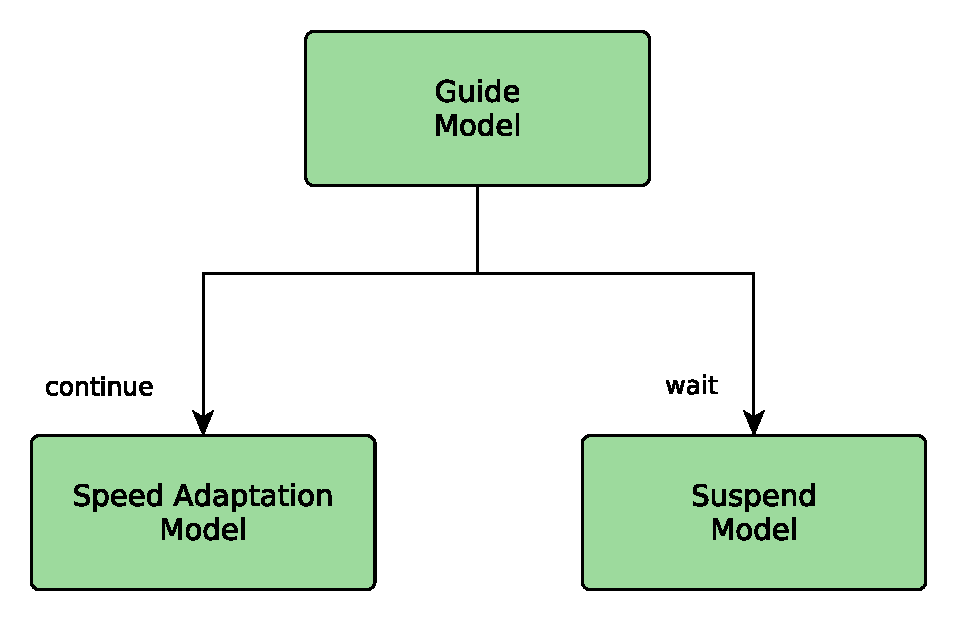
\includegraphics[scale=0.45]{img/case_study/spencer/guide_planner.pdf}
	\caption[Collaborative planner for guiding]{This figure shows the hierarchical MOMDP collaborative planner use to guide a Group. The arrows show the macro-actions of the root of the hierarchy, leading to sub MOMDPs.}
	\label{fig:case_study-spencer-guide_planner}
\end{figure}

\subsection{Representing a group}
Our system has been built with the assumption that the robot would navigate in a crowded environment, where its followers could be often occluded. In addition, after speaking with our partners, we understood that the perception components would not be able to maintain a stable identifier for members of the groups, meaning that the robot would not be able to realiably understand if a group of users is following it. We tried to maintain a good balance between accuracy, trying to guide effective users and not people whose which are going in the same direction as the robot, and robustness, copying with unreliable perception.

We built our collaborative planner following these ideas:
\begin{itemize}
\item The robot will record a list $g$ composed by the identifiers of the group at the start of the scenario. During this scenario, it will maintain a list $f$, composed by users that are still tracked whose identifier is in $g$, and another list $o$, composed by all the tracked people whose distance from the robot is less than a costant $d$. 
\item As long as $f$ is not empty, the robot will choose a \textit{best} follower $b$ from this list, and try to guide him, using the collaborative planner. The \textit{best} follower is chosen by considering the user whose behavior is the most consistent with the robot, by taking into account the speed, distance and orientation of the user.
\item If $f$ is empty, but $o$ is not, the robot will choose a \textit{best} follower $b$ from $o$, and try to guide him, using the collaborative planners.
\item If  both $f$ and $o$ are empty, the robot will abandon the task.
\end{itemize}

Our idea is considering that the robot's followers will \textit{act as a group}, staying together as much as they can. The robot will try to guide members of the group, but if it has lost tracking of all of them, and there is still somebody behind it which is acting in a consistent way with the guiding task, it will think that its users are still following it, but their identifiers have changed in the perception layer.


\subsubsection{Guiding a User}
The main problem of the robot is choosing if it should still guide the group, suspend temporarily the task, or abandon it. The Guide Model is the root MOMDP of our architecture and will make this decision, based on three main variables: 
\begin{itemize}
\item The status of advancement of the task. This variable, whose values are \textit{\{not\_completed, completed\}}, is set by the Action Executor module, in the Execution Management layer, depending on the current advancement of the task. The variable will be set as $not\_completed$ until the robot as reached the final destination in the plan. 
\item The quality of commitment of the group. This variable, whose values are \textit{\{not\_engaged, engaged, not\_interested\}}, is hidden, estimated from observations produced by the Situation Assessment layer. The observations used are: the distance of the user from the robot, its variation, the orientation of the user in respect of the  robot, and if the user is currently moving or still. We expect engaged users to have a behavior that is coherent with the task, moving to follow the robot and taking a similar path. Users are considered not engaged when they stop following, perhaps even disappearing from the robot's sight. Finally, we infer that users are not interested in following the robot if they have been \textit{not\_engaged}  for too long.
\item A timer. This variable can assume the values \textit{\{not\_expired, expired\}}. When a user is detected as $not\_engaged$, the Action Executor starts a timer. When this timer expires, the value of this variable is set accordingly.
\end{itemize}

The Guide Model can execute the following actions:
\begin{itemize}
\item $Continue$. A macro-action, which leads to the Speed Adaptation Model.
\item $Wait$. A macro-action, which leads to the Suspend Model.
\item $Abandon$. Signals the Action Executor to abandon the current task.
\end{itemize}

\subsubsection{Adapting the Robot's Speed}
We believe that to be socially acceptable, the robot should adapt its speed to his follower. By setting its own pace at the start of the scenario the robot  would risk of being too slow, annoying users, or too fast, which would lead the robot to constantly stop to wait for users, producing an awkward behavior. Adapting to users might not be enough in some tasks, and, depending on the situation, the robot might desire to influence the behavior of its follower, to respect social rules or to accomplish its task in a more efficient way. Its important to find a balance between these two behaviors, which is the goal of the Speed Adaptation Module. 

To adapt to the speed of the group, the robot defines a desired range of distances $[dr_1,dr_2]$ from the best follower $b$. The distance of $b$ from the robot, $d(b,r)$ will influence the chosen action:
\begin{itemize}
\item if $d(b,r)>dr_2$  the model will influence the robot to \textit{decelerate}.
\item if $d(b,r)<dr_1$ the model will influence the robot to \textit{accelerate}.
\item if $dr_1<d(b,r)<dr_2$ the model will influence the robot to maintain its current speed.
\end{itemize} 

In our study, $dr_1$ and $dr_2$ were predefined values, but they could be learnt and adapted to the users during the task, since different people could prefer following the robot at different distances and positions.

The robot should also not constantly change speed, in order to give time to users to adapt to its new chosen speed, and so we defined a temporal threshold in which we do not allow the robot to repeat an \textit{accelerate} or \textit{decelerate} action.

We studied two different situations where the robot can proactively try to influence the speed of the group.
\begin{itemize}
\item There is a time limit to reach the destination. In this case the robot must balance the desire to satisfy the group with the task urgency. Different situations will require different policies. For example, in an airport scenario, the robot could prioritize arriving on time, warning users if their speed would render the goal not achievable, while in other situations the robot could try to arrive in time but still avoid to adopt speeds that are uncomfortable for the group.
\item The rules of the current environment limit the robot's speed. In this case the robot will avoid accelerating over a set speed even if it detects that its current velocity is considered too slow for the group. For example, the robot could be navigating in a construction zone.
\end{itemize}

\subsubsection{Suspending the task}
In some situation, the robot needs to suspend the task, because the group has stopped following it. In this case, the robot should estimate if this suspension of the collaborative scenario is temporary or permanent, and in the latter case abandon the task. We estimate this information using the Suspend Model and the activity areas from Situation Assessment. We link activity areas to the maximum time we expect that the group will be involved in the linked activity, and with a set of proactive actions that the robot can choose to execute.

In our work, we investigated a single possible proactive behavior: giving information. In this case, if we detect that one or more  members
of the group has stopped following because it is looking at a touristic sight, or at an information screen, the robot can try to engage him and offer related information. At the moment, we just propose a simple routine-based framework for this behavior, and plan to further study it in the future. We believe that the solution of this problem could be rich, and that the robot should estimate the reaction of the group during the execution of its proactive behavior, in order to be able to interrupt if the group does not want to be helped or to resume the original task if they are satisfied by the robot's actions.

We do not want the robot to be inactive for a long time  waiting for the group. If there is a small amount of time to reach the destination, or the group is engaged in the activity for a longer period of time than the one predicted, or the robot can not estimate the reason why the group stopped following, the Suspend Model can issue a warning action, and eventually abandon the task if the group does not start following it again.



\subsection{Laboratory Experiments and Analysis}
\label{subsec:case_study-spencer-lab_experiments}

To have a first validation of our system, we performed experiments in a laboratory.

In this setting, we used Motion Capture to track users, and a navigation software based on \cite{sisbotTRO2007,kruse12crossing}. This software add proxemics based costs to static humans in the environment, continuously predicting and avoiding future collisions with moving persons, while  simultaneously keeping the robot as close as possible to the planned path.

\begin{figure}[ht!]
	\centering
	\includegraphics[scale=0.2]{img/case_study/spencer/robotGuiding.png}
	\caption[Robot Guide laboratory experiment]{This figure shows the SPENCER robot guiding a user in a laboratory}
	\label{fig:case_study-spencer-robotGuiding}
\end{figure}

We performed experiments with a single user following a robot on a predefined path. Data from these experiments are shown in table \ref{table:case-study-spencer-experiment_results} and in figure \ref{fig:case_study-spencer-exp_lab_result}. We start by showing speed adaptation tests:
\begin{itemize}
\item \textit{Adapting slow and fast}. In these two tests (figure \ref{fig:case_study-spencer-robotGuiding}) we used our system to guide respectively a user that would like to move at a slow pace, and a user that would like to move at a fast speed.
\item \textit{No adaptation}. In this experiments the robot will not adapt to the speed of the user, setting its own pace and stopping if it is too far.
\end{itemize}

Looking at the data we can see that our system shows lower values for the variance of speed and distance, which means that after a certain time it is able to find a condition of equilibrium with the human follower. The \textit{no adaptation} system shows a significantly higher variance for both values, since the robot stopped several times to wait for a user. We will now show some tests regarding the proactive behaviors of the robot:

\begin{itemize}
\item \textit{Proactive slow and fast}. During the task, the robot proactively chooses to change pace, in the first case by slowing down and in the second by accelerating. In our tests the user adapted after some seconds to the robot's pace, but this behaviors should be studied in-depth in user studies.
\item \textit{Suspend with screen and with no reason}. In these tests we asked a user to stop during the task. In the first case the user stopped near an information screen. After detecting this event, the robot approached the user to offer information, which lead to the resumption of the task. In the second case the user stopped at a different point of the path. The robot was not able to detect the reason for the suspension of the task and so simply   issued a warning to the user, abandoning the task after some seconds.
\end{itemize}


\begin{table}
\caption[Experiment results on speed adaptation]{Experiment results: $d$ is the distance between the robot and the user, $s_r$ is the robot's speed, $s_h$ is the human's speed, $\mu$ is the average and $\Delta$ is the variation of the quantity. Distances are expressed in meters, velocities in meters for seconds.}
\centering
\begin{tabular}{ | c | c | c | c | c | }

\hline
  test name     & $\mu$ $distance$ & $\mu$ $speed$ $difference$ & $\Delta$ $distance$ & $\Delta$ $speed$ $difference$ \\
\hline
adapting slow & 2.82 & -0.03 & 0.64 & 0.02 \\
  \hline
  adapting fast & 1.38 & 0.00 & 0.29 & 0.01 \\
  \hline
  no adaptation & 3.08 & -0.09 & 1.04 & 0.07 \\
\hline
proactive slow & 1.45 & -0.06 & 0.04 & 0.10 \\
\hline
proactive fast & 2.66 & -0.11 & 0.63 & 0.01 \\
\hline
\end{tabular}
\label{table:case-study-spencer-experiment_results}
\end{table}

\begin{figure}[ht!]
	\centering
	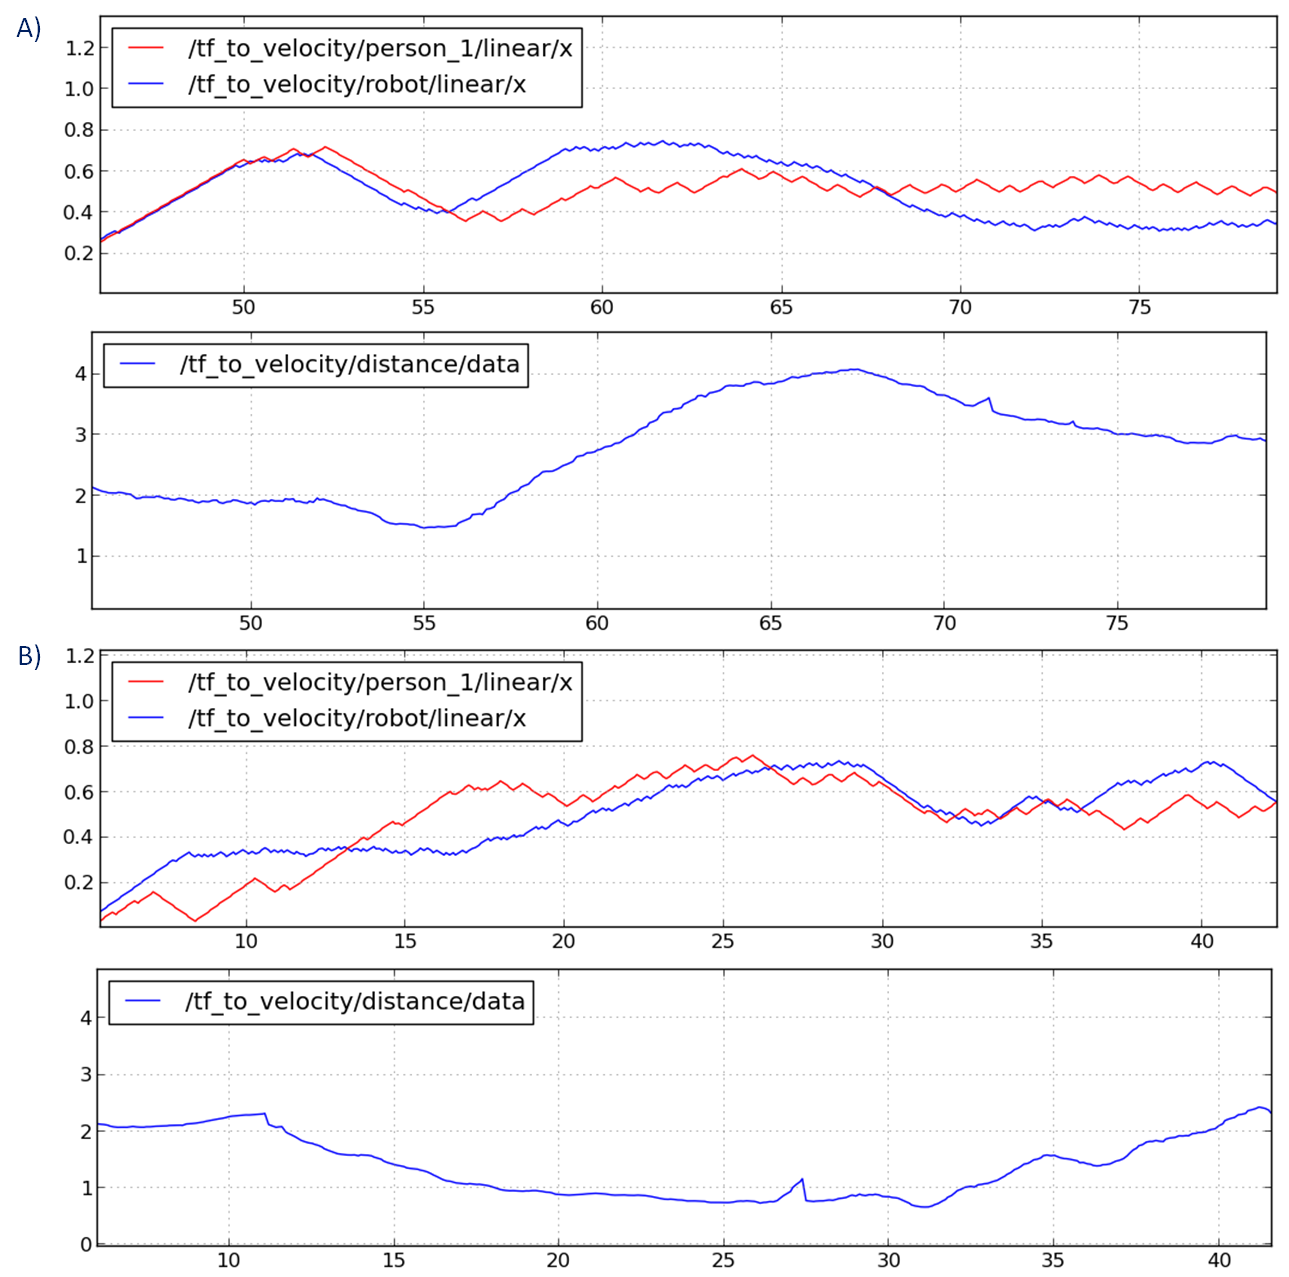
\includegraphics[scale=0.5]{img/case_study/spencer/experiments.png}
	\caption[Robot Guide laboratory experiment]{Robot Guide Laboratory Experiments: a) Adapting robot speed to a slow user. The first figure shows the speed of the user ($tf\_to\_velocity/person\_1/linear/x$) and of the robot ($tf\_to\_velocity/robot/linear/x$), and the second their distance. The robot starts slowing down at $t=60$, when the distance from the user is growing, until it finds an equilibrium with the user's speed. Notice that there is a turn in the path, at $T=50$, that causes the robot and the user to slow down. Distances are expressed in meters, velocities in meters for seconds.
b) Adapting robot speed to a fast user. As before, the figures show the robot and user's speed and their distance. The robot starts accelerating at $t=15$  when the distance from the user becomes small.}
	\label{fig:case_study-spencer-exp_lab_result}
\end{figure}

\subsection{Results on Airport Deployment}
\label{subsec:case_study-spencer-airport}
\subsubsection{Integration with Other Components}
The system was deployed in the Schiphol Airport for two different sessions, respectively of a week and of two weeks. In those weeks the team of the SPENCER project adapted the robot to the complex environment of the airport. Our system was integrated with several softwares from our partners, such as a combined laser-RGB people tracker, developed in \cite{lindermulti}, a novel localization approach, shown in \cite{kucner2015ndt}, a RTT based motion planner, shown in \cite{palmierirrt}, and cost-based social rules, introduced in \cite{okallearning}. More details on the whole SPENCER system are available in \cite{triebel2015spencer}.


\begin{figure}[ht!]
	\centering
	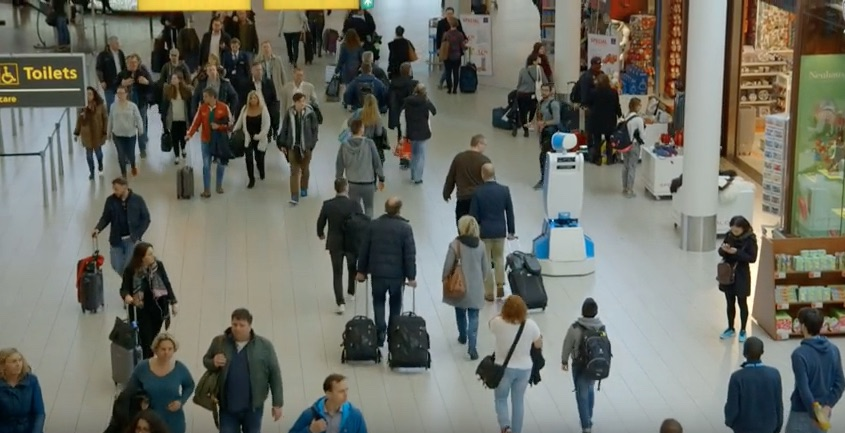
\includegraphics[scale=0.45]{img/case_study/spencer/spencer_schiphol.png}
	\caption{The robot moving in the Schipol airport}
	\label{fig:case_study-spencer-spencer_moving}
\end{figure}


\begin{figure}[ht!]
	\centering
	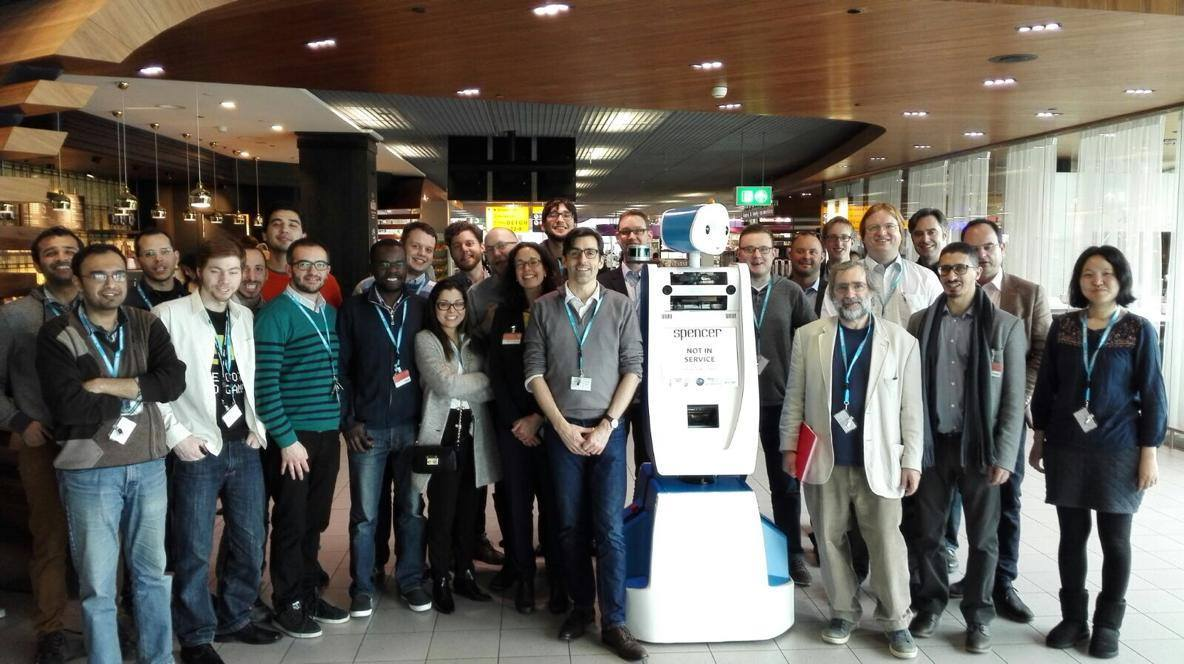
\includegraphics[scale=0.45]{img/case_study/spencer/all.jpg}
	\caption{The team that worked on the SPENCER project.}
	\label{fig:case_study-spencer-team}
\end{figure}

\subsubsection{User Study}

The system was tested in a user study, performed by researchers of the University of Twente\footnote{https://www.utwente.nl/en/}, which participated in the project. The study was conducted in two different days, with 18 participants, 11 males and 7 females, aged between 26 and 54. Ten participants indicated that the purpose of their journey was business, while eight indicated pleasure. Two different tests were performed:

\begin{itemize} 
\item In the first test the robot would pick up users at a chosen point, in Lounge-1 or in the Starbucks coffee shop of the airport, and guide them to a prefixed gate, B18. Users interacted with the robot by scanning special boarding passes created for this test on the robot's board pass reader, which prompted the start of the mission. To reach the gate, the robot had to pass through a crowded area, composed by several shops and other flight gates.
\item In the second test the robot met users at the gate B18 and guided them to Lounge-1. In this situation users initiated the mission by using the touchscreen display of the robot to select the destination.
\end{itemize}

At the end of each test, we collected three different kind of measures:
\begin{enumerate}
\item An individual feedback questionnaire where the users evaluated several aspects of the robot, like its behavior and aspect, on a 7-point Likert scale. In the day of testing two new questions where introduced about the robot, and a question on the participant's opinion on the robot in general.
\item A group interview, where users could discuss about their first impression of the robot, their experience in the test, and their thoughts on how to improve the systemm.
\item  Notes taken by researchers during guide, that helped to contextualize the results of users and to record specific events that occurred during tests.
\end{enumerate}


\begin{figure}[tb]
  \begin{center}
  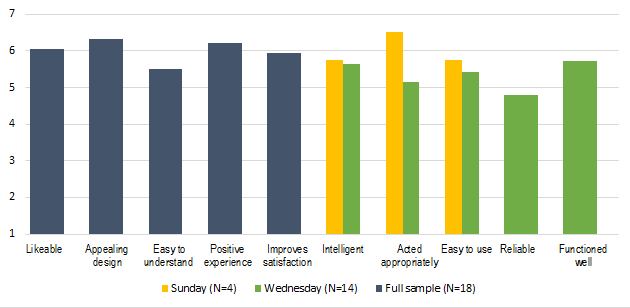
\includegraphics[width=0.95\textwidth]{img/case_study/spencer/graph_subjective_questions.png}
  \end{center}
  \caption{Answers to feedback questionnaire}
  \label{fig:feedback_questionnaire}
\end{figure}


Figure~\ref{fig:feedback_questionnaire} shows the results of the feedback questionnaire. Two questions were reformulated between the two days of testing, and so we included means for both of them. While the number of tests conducted were too limited to generalize, we can affirm that the participants had in general a positive impression of the robot. We list the main results of this test.

\begin{itemize}
\item Participants were generally happy with the robot's guiding performance.
\item The robot can be described as friendly-looking, easy-to-use and reliable.
\item The main issues encountered by users where related to the boarding card reader of the robot, and to its frequent abrupt stoppings.
\item Some users considered the speed of the robot too fast, or too slow, for their experience.
\item Users thought that the robot guide could be useful for people inexperience with flying, or new to a particular airport.
\item Users thought that the robot improved their customer satisfaction.
\item The main improvements for the robot include technical improvements, in particular related to the frequent stopping, and the addition of new functionalities, like carrying luggage or guiding to shops and restrooms.
\end{itemize}

\subsubsection{Discussion}
The experience in the airport showed the complexity of deploying a robot in such a complex scenario, interacting with inexperienced users. From our experiments we noticed several things:
\begin{itemize}
\item It is important to not make too many assumption about how users will interact with the robot. We expected users to follow the robot, staying mostly on its rear or side regions. This was not always true. In fact, several users were more interested in moving ahead of the robot, often concentrating on its behaviors more than on following it. The robot should adapt to these behaviors and not consider them as errors.
\item Human-Aware motion in complex environments is still a hard problem. Adapting the robot's speed was not simple, because the robot had stop or slow down often to avoid obstacles. Some times false positives generated by perception can lead to abrupt stops by the robot, which are seen as annoying and unnatural by users, and could even be dangerous.
\item Users are fascinated by robots, and are willing to ignore errors generated by the systems in short-term experiences.
\item It is important to perform long deployments in similar scenarios with real users. A long time in the three weeks where we worked at the airport was spent adapting the robot to the scenario. Longer deployments would allow for an iterative process of design-implementation-study.
\end{itemize}
